\documentclass[a4paper, 12pt]{article}
\usepackage{graphicx}
\graphicspath{{assets/}}
\begin{document}
\title{\textbf{ANDROID AUTO}}
\date{}
\maketitle
\paragraph{Google, Apple and car companies are in a relentless
three-way-tug-of-war for control of your dashboard. Automakers generally prefer motorists use their car's native software, but the ricvaling technology giants offer more alternatives that are better packaged. Googles proprietory projection standard is} \textbf{Android Auto}
\paragraph{\textbf{WHAT DOES ANDROID AUTO DO?}}
\subparagraph{Android Auto takes the features you love about your android-powered smartphones and puts them directly into your car's dashboard}
\subparagraph{One of the best parts of Android Auto is the Google Maps-powered navigation system, which provides step-by-step directions and automatically finds an alternate route if it detects heavy traffic.\\
It also ports over saved destinations, so you don't have to manually type "home", "work", or your other favourite destinations.}
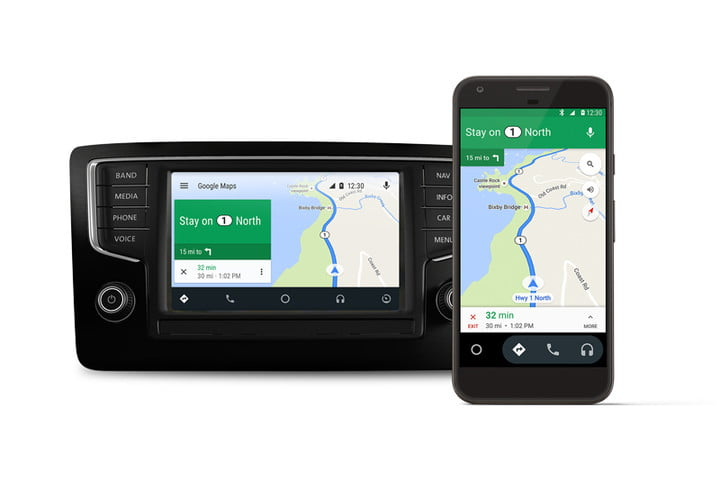
\includegraphics[width=\textwidth]{map}
\textbf{Figure 1:} Shows the interaction of an android phone, Android Auto with Google Maps
\subparagraph{The software also gives motorists on-demand access to million of songs
and podcasts, lets them surf the web, and allows them to stay connected via calls and messages.}
\subparagraph{Android Auto also works with a set of third-party apps, including Pandora, Iheart, Skype, WhatsApp, Spotify and others. However, vehicle settings aren't part of Android Auto, so the driver has to exit the application to adjust climate controls, browse radio stations, or select a different driving mode. But google is currently working with carmakers to create new Android-based systems where all these features will be accessible from one place.}
\paragraph{\textbf{WHICH PHONES ARE COMPATIBLE WITH ANDROID AUTO?}}
\subparagraph{Android Auto works with all Android-powered phones that run 5.5(Lollipop) or higher. In order to use it, you will need to download the free Android Auto Appand connect your phone to your car using a USB cable. Google promises wireless support will be available in the not-too-distant future, but it's not yet available.}
\paragraph{\textbf{WHICH CARS ARE COMPATIBLE WITH ANDROID AUTO?}}
\subparagraph{There are a dozen of cars that support Android Auto. However, some car manufacturers charge buyers extra for the feature while otherschoose not to offer it on a cheap trim levels.}
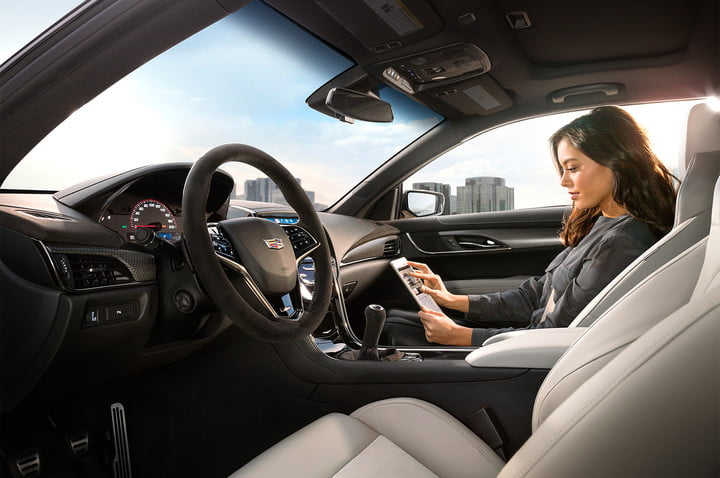
\includegraphics[width=\textwidth]{car}
\textbf{Figure 2:}Android Auto-Compatible Car
\subparagraph{Android Auto-compatible cars include most members of Mercedes-Benz lineup, Honda, Volvo, Volkswagen, and others}
\subparagraph{The exception to the rule is Toyota, which continues to resist Android Auto and Apple's rival software Carplay due to safety and private concerns.}
\paragraph{\textbf{HOW TO CONNECT YOUR PHONE TO ANDROID AUTO?}}
\subparagraph{Whether you've purchased a vehicle equipped with Android Auto from the factory or found a suitable aftermarket system that includes the software,  you will need to connect your device. Here is how to get the software up and running.}
\subsection{Assure your phone is running android 5.0(Lollipop) or a newer operating system and you have downloaded Android Auto for both your phone and device, and that you have a strong LTE or WiFi connection.}
\subsection{With your vehicle in Park, turn your car and phone on, plug in your phone via USB, and review the Safet Notice and Terms and Conditions. Alternatively you can pair yur device via bluetooth.}
\subsection{Follow on-screen steps to give Android Auto permission to access your phone;s features and apps.}
\subsection{On your car's display, select Android Auto app and follow the instructions to get started.}
\subparagraph{Once you have connected your device, you'll have Android Auto's convenient features for smarter and safer driving.}
\end{document}